\documentclass[11pt]{article}

\usepackage{amsmath}
\usepackage{textcomp}
\usepackage{tikz}
\usepackage[top=0.8in, bottom=0.8in, left=0.8in, right=0.8in]{geometry}
% add other packages here

% put your group number and names in the author field
\title{\bf Exercise 2: A Reactive Agent for the Pickup and Delivery Problem}
\author{Group \textnumero 17: Ogier Bouvier, Val\'erian Rousset}

% the report should not be longer than 3 pages

\begin{document}
\maketitle

\section{Problem Representation}

\subsection{Representation Description}
% describe how you design the state representation, the possible actions, the reward table and the probability transition table

We generate a possible set of states, each with either

\begin{itemize}
	\item The current city, a task and the destination city of the task.
	\item The current city and without a task.
\end{itemize}

From each of these state we have two possibilities

\begin{itemize}
	\item If we have a task, move to the destination city.
	\item If we don't have a task, we go to the neighbooring city which
		has the best potential reward, the reward of a package minus
		the cost of travelling there. Cost itself is defined by the
		distance to the city times the cost per kilometer.
\end{itemize}

\subsection{Implementation Details}
% describe the implementation details of the representations above and the implementation details of the reinforcement learning algorithm you implemented

For each possible state, we find the possible actions (for exemple, we can't
deliver if we don't have a task), then for each, we compute the best
reward weighted by the probability of  and add it to the generated
map. Then, we do it over and over (for each path in the state graph),
until the map stabilize, meaning that we have reached the optimal
value for every state.

\section{Results}
% in this section, you describe several results from the experiments with your reactive agent

\subsection{Experiment 1: Discount factor}
% the purpose of this experiment is to understand how the discount factor influences the result

\subsubsection{Setting}
We tested using three different discount factor. One agent runs with a
discount factor of 0.20, another 0.60 and the last 0.90.

We tried two parameters, one with discount factor of 0.01 and one with discount
factor of 0.85.

It was simply set by editing the config/agent.xml file.

\subsubsection{Observations}
\begin{figure}
  \caption{Simulation result for the three different settings}
  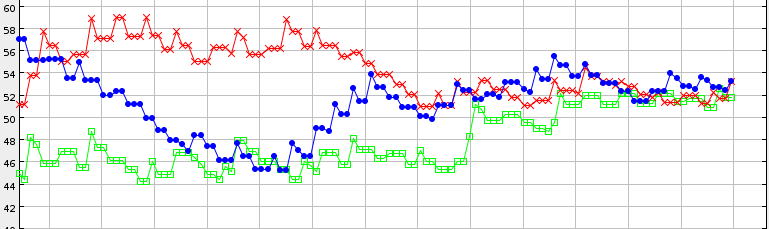
\includegraphics{compare_discount}
  \centering
\end{figure}

\begin{itemize}
	\item 0.85
\end{itemize}

\subsection{Experiment 2: Comparisons with dummy agents}
% you compare the results of your agent with two dummy agents: the random agent that was already given in the starter files and another dummy agent that you define and create. You should report the results from the simulations using the topologies given in the starter files and optionally, additional topologies that you create.

\subsubsection{Setting}
We have implemented a dumb agent which is basically the same as the
Random agent except it always picks up task when one is available. If
not it will move to random neighbor of the current city.

We run all 3 agents in one simulation. The first two have a discount
factor of 0.85 and the second one has no parameter.

\subsubsection{Observations}
\begin{figure}
  \caption{Simulation result for the 3 agents comparison}
  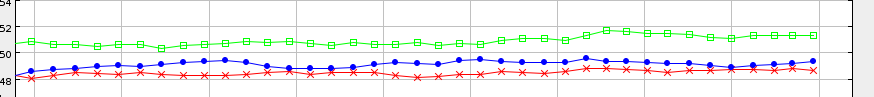
\includegraphics{compare_3}
\end{figure}
% elaborate on the observed results

\end{document}
